\documentclass{report}
\usepackage{setspace} % Setting line spacing
\usepackage{ulem} % Underline
\usepackage{caption} % Captioning figures
\usepackage{subcaption} % Subfigures
\usepackage{geometry} % Page layout
\usepackage{multicol} % Columned pages
\usepackage{array,etoolbox}
\usepackage{fancyhdr}
\usepackage{enumitem}
\usepackage[toc,page]{appendix}

% Page layout (margins, size, line spacing)
\geometry{letterpaper, left=1in, right=1in, bottom=1in, top=1in}
\setstretch{1.5}

% Headers
\pagestyle{fancy}
\lhead{PeaPod - Design Proposal}
\rhead{UTAG}

% Metric counter, referencing commands
\newcounter{metricnumber}
\setcounter{metricnumber}{1}
\newcommand{\metricrow}{M\arabic{metricnumber}}
\newcommand{\mlabel}[1]{\addtocounter{metricnumber}{-1}\refstepcounter{metricnumber}\label{#1}\addtocounter{metricnumber}{1}}
\newcommand{\mref}[1]{M\ref{#1}}

\begin{document}

\begin{titlepage}
    \begin{center}
        \vspace*{1.2cm}

        \textbf{\large{PeaPod - Design Proposal}}

        \vspace{0.5cm}

        Outlining a Proposal to the PeaPod Design Brief

        \vfill

        Jayden Lefebvre - Lead Engineer\\\small{jayden.lefebvre@mail.utoronto.ca}\\
        \vspace{1cm}
        Nathan Chareunsouk, Navin Vanderwert, Chris Lansdale - Design Engineers

        \vspace{2.5cm}

        Revision 0.2\\
        University of Toronto Agritech\\
        June 4th, 2021

    \end{center}
\end{titlepage}

\thispagestyle{plain}

\tableofcontents
\newpage

\section{Introduction}
\label{sec:intro}

\subsection{Purpose}
\label{sec:purpose}

The purpose of this document is to outline the fuction and features of a proposal to the PeaPod Design Brief.

It accomplishes this by answering the following questions on a recursively-scoping basis:
\begin{enumerate}
    \item \textbf{What} is the design? What does it accomplish/what is its function? 
    \item \textbf{How} does it accomplish this? What are its features? 
    \item \textbf{Why} that functionality? Why that way?
\end{enumerate}

\newpage

\section{Design}

Functions of the design are derived from the input and output requirements.

\begin{figure}[h]
    \centering
    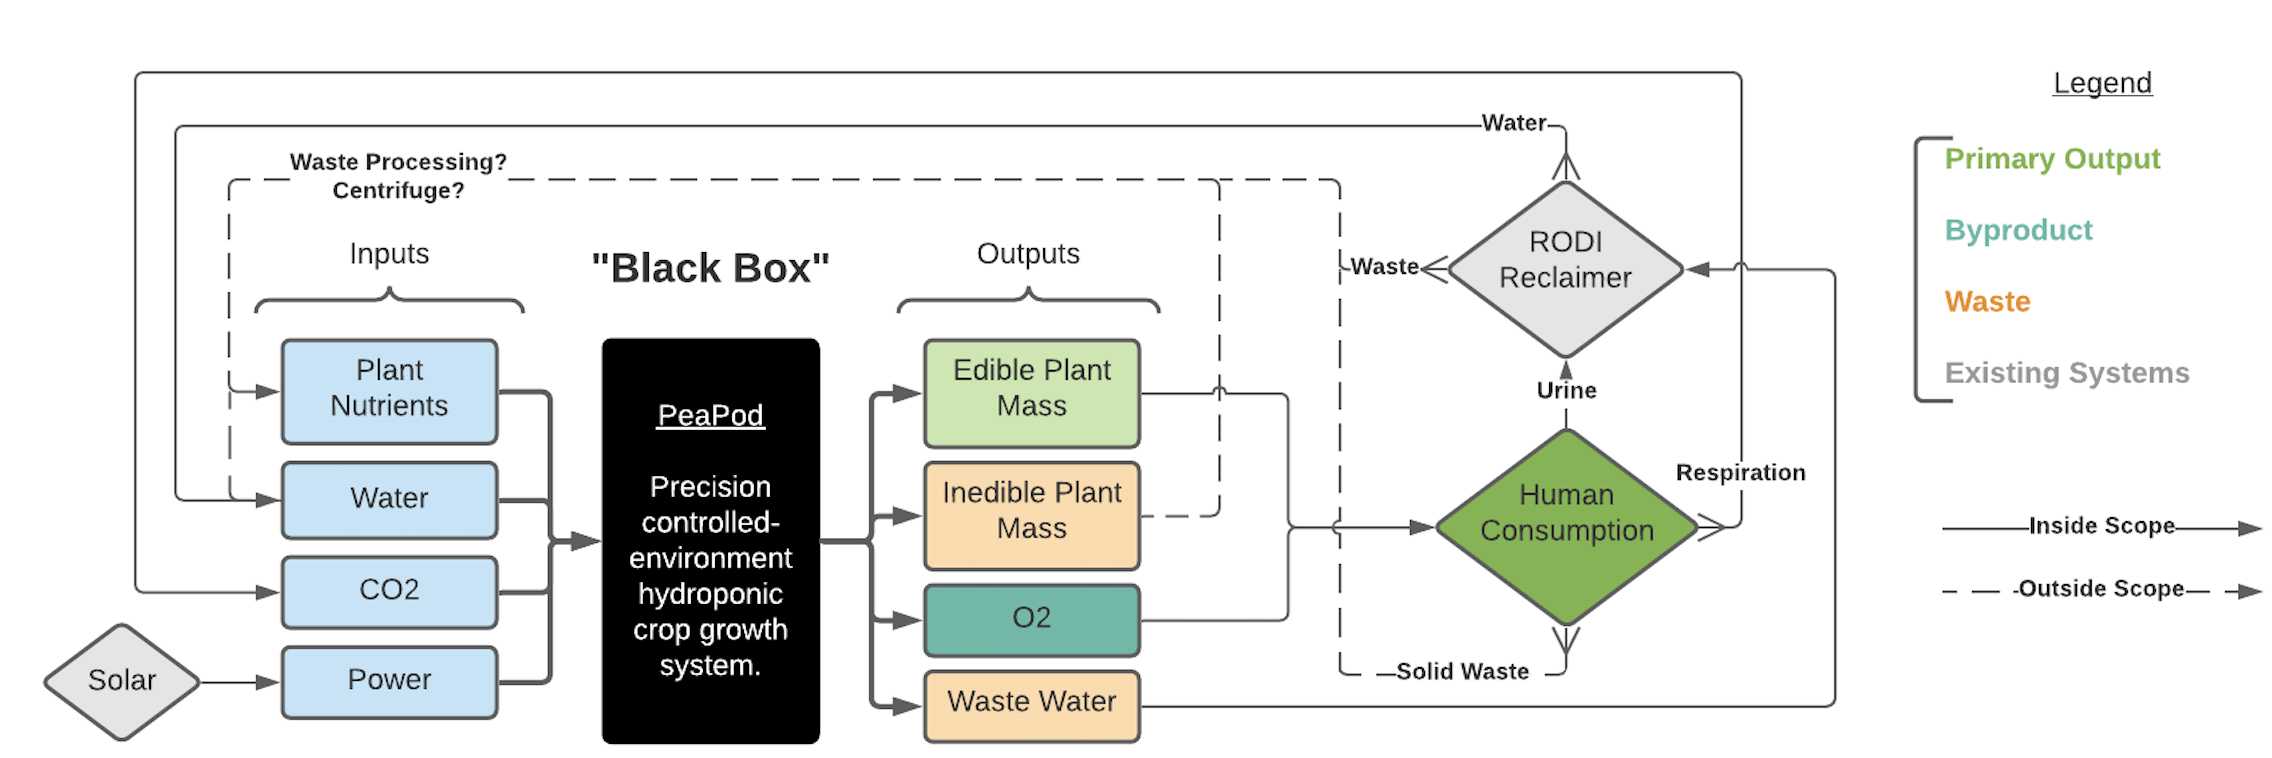
\includegraphics[width=15cm]{images/blackbox.png}
    \hfill
    \caption{"Black box" input-output model of PeaPod.}
\end{figure}

Features of the design are developed to meet the function, and are derived from the opportunity statement:

PeaPod is "an \uline{automated} and \uline{isolated} \uline{aeroponic} crop growth system, able to generate any environment from a combination of independent \uline{environment parameters}, with both environment and crop growth \uline{data collection}".

\begin{figure}[h]
    \centering
    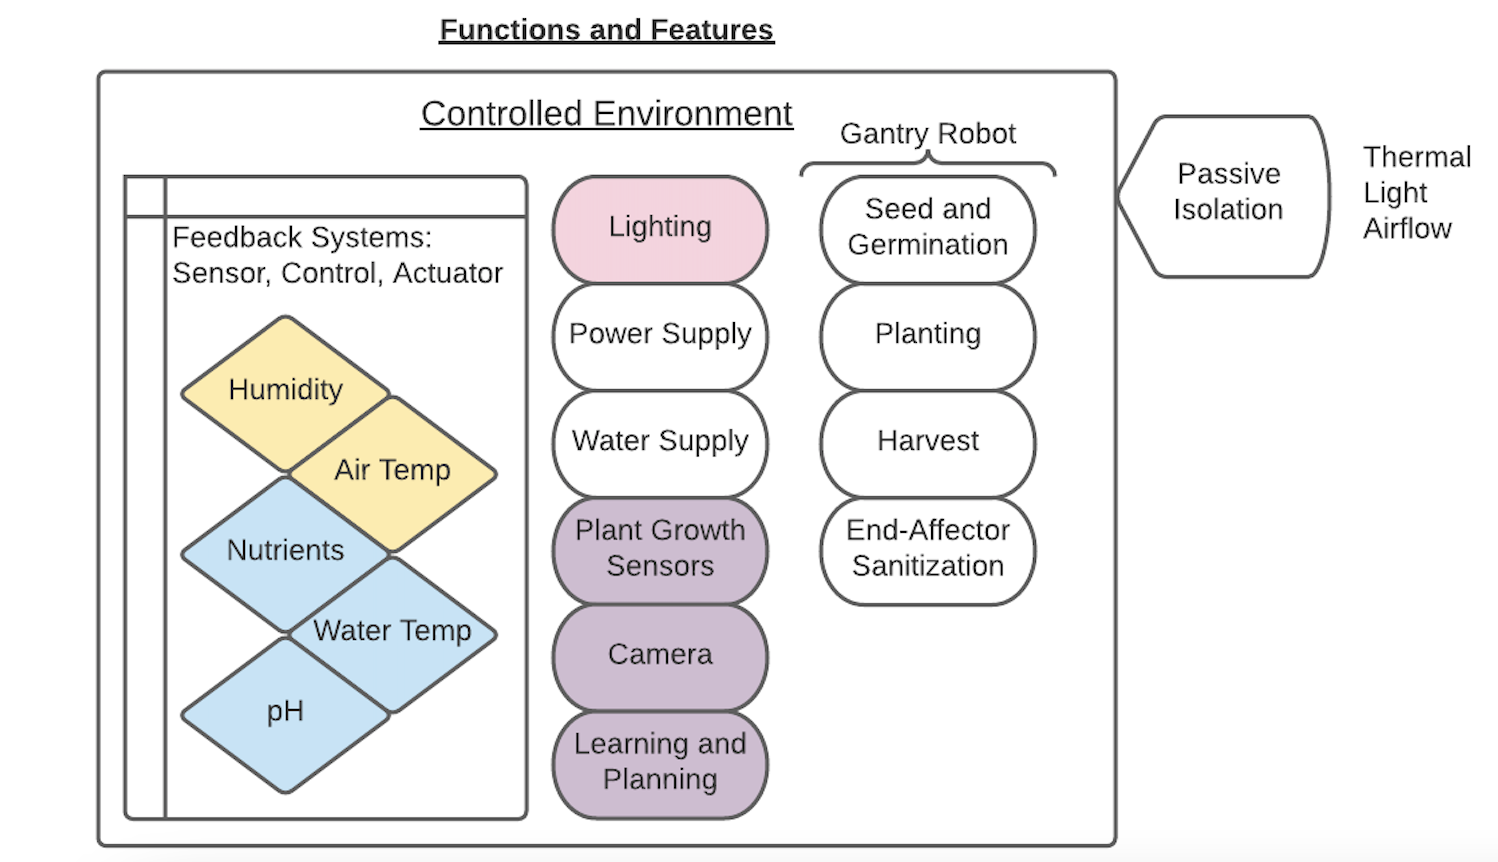
\includegraphics[width=12cm]{images/features.png}
    \hfill
    \caption{Features and feature types of PeaPod.}
\end{figure}

\newpage

\subsection{Automation}
\label{sec:automation}


\textbf{What}: Performing growth-, maintenance-, and data-related tasks autonomously on the basis of both schedule and necessity.

\textbf{How}:
\begin{itemize}
    \item Schedule:
    \begin{itemize}
        \item User inputs time/action pairs
        \item E.g. Water at 08:00, Turn light to setting X at 14:00
        \item \textit{Bonus:} Can notify user if action's resource is missing (i.e. water tank low)
    \end{itemize}
    \item Necessity:
    \begin{itemize}
        \item "Sense, Plan, Act" robotics/control model:
        \begin{enumerate}
            \item \textit{Senses} current conditions
            \item \textit{Plans} a path to desired condition
            \item \textit{Acts} to change current condition to desired condition
        \end{enumerate}
    \end{itemize}
\end{itemize}
\textbf{Why}: Increase accuracy/precision, minimize human hours spent

\subsection{Isolation/Insulation and Housing}
\label{sec:isolationinsulation}

\textbf{What}: Isolates the growth environment from the exterior environment, provides structural integrity and mounting points.

\textbf{How}: Cube exoskeleton (aluminum extrusion) holds solid (acrylic/foam/corrugated board) interenally-reflective (mylar) panels in place and aids in mounting plant growth platforms, lights, etc.

\textbf{Why}: Increases thermal and light efficiency. Isolation increases safety against cross-contamination, pathogens, harmful substances. Simple and strong construction with dedicated mounting channels.

\subsection{Aeroponics}
\label{sec:aeroponics}

\textbf{What}: Medium-free growing method that uses nutrients dissolved within atomized water

\textbf{How}: High-pressure (pump-tank-switch system) nozzles deliver atomized ($\approx$50 micron droplet) nutrient solution to plant roots. Parallel distribution topology (T-quick-connects at every unit height, solenoid ball valves at tank out and in each tray)

\textbf{Why}: No water parameter feedback, 98\% more water efficient, minimizes pathogens and waste water

\newpage

\subsection{Environment Control}
\label{sec:environment}

The environment control feature can be broken up into \textbf{control systems} (\ref{sec:airtemp}-\ref{sec:dehum}; sometimes in two parts) and \textbf{set systems} (\ref{sec:watertemp}-\ref{sec:lighting}).

\subsubsection{Air Temperature}
\label{sec:airtemp}

\textbf{What}: Maintaining desired air temperature within the enclosure

\textbf{How}: Thermoelectric heating/cooling system (peltier tiles w/ polarity switch and 'dimming' current control) on a heat sink w/ fan

\textbf{Why}: Better space and energy efficiency, less complexity (no liquids, pressurized fluids, etc.), better control

\subsubsection{Air Humidification}
\label{sec:airhum}

\textbf{What}: Adding water vapour to air

\textbf{How}: Ultrasonic nebulizer (piezo disc w/ custom driver circuit), RO water

\textbf{Why}: Piezo for droplet size, commonly used; RO for purity of water vapour

\subsubsection{Air Dehumidification}
\label{sec:dehum}

\textbf{What}: Absorbs water vapour from the air

\textbf{How}: Silica gel beads, controlling airflow rate across

\textbf{Why}: Non-toxic, safe, cheap, effective. Color-changing indication at saturation, easily reset by baking and recapturing water

\subsubsection{Solution Temperature}
\label{sec:watertemp}

\textbf{What}: Maintaining desired water temperature within the water store

\textbf{How}: Same as \ref{sec:airtemp}; on a water block

\textbf{Why}: Same as \ref{sec:airtemp}

\newpage

\subsubsection{Solution Nutrients}
\label{sec:nutrients}

\textbf{What}: Precisely dosing the correct amount of nutrients to the water system at setup/water addition

\textbf{How}: Syringe dosage via servo motor to set ppm based on fill volume

\textbf{Why}: Syringe dosage is precise, easy to refill

\subsubsection{Solution pH}
\label{sec:ph}

\textbf{What}: Precisely adds pH up/down solutions to set the solution pH at setup/water addition

\textbf{How}: Same as \ref{sec:nutrients}

\textbf{Why}: Same as \ref{sec:nutrients}

\subsubsection{Lighting}
\label{sec:lighting}

\textbf{What}: Wide spectrum precision LED lighting targeting PAR

\textbf{How}: N LED series/colors, N controlled-current PWM drivers, M LEDs per series = NxM LEDs. Custom LED boards wired in series, one power board per tray, w/ diffusion

\textbf{Why}: LED > every other type in every way, PWM easy protocol, CC because they’re LEDs

% \textbf{What}: 
% \textbf{How}: 
% \textbf{Why}:

% \newpage

% \textbf{What}: 
% \textbf{How}: 
% \textbf{Why}:

% References
% \bibliographystyle{IEEEtran}
% \bibliography{references}
\end{document}